Moreover this level crossing ADC tracks the analog input in linear fashion. as a result when the analog input changes rapidly the slopeover load error goes on increasing, which makes the level crossing ADC useless for high frequency signals.

	The proposed architecutre is desigened in such a way that the loop delay is reduced by changing up-down counter with a more intilligent controller circuit when the analog input changes rapidly. Which tracks the analog input in more intilligent manner. The operation of Contrroller is shown in Fig.~\ref{fig:FLOWCHART} as a flow chart for 8-bit hardwear resolution. \par

	The proposed controller tracks the analog input in logarathmic fashion rather then linear fashion which is generally followed in conventional LC-ADC's. At maximum the proposed LC-ADC takes $2N$ clock cycles for complete the process if the analog input changes from minimum to maximum, where as the conventional LC-ADC's which use up-down counter will take $2^N$ clock cycles to complete the operation when the analog input changes from minimum to maximum value.\par



	The controller works as follows, when a trigger signal genreted by the difference quantificator, the controller checks for which signal it is, If it is a $INC$ signal then it chcks for a '0' from LSB to MSB, if it finds a 0 at LSB then changes LSB from 0 to 1, it effectively implies as increasing the present data by 1. If it does find 0 in LSB, it checks next bit to LSB, untill it finds a 0. Then it changes the 0 into 1 and applies to the capacitor array to fix the as in conventional SAR ADC's. It uses the same DAC which is used to generate the reference signal for difference quantificator.\par

	The intialization process ends when the refence signal $V_{ref}$ is greater then $V_{inp}$ at this point of time the bits from current position to LSB all will be set to '1'. Then the bits from LSB to 1-bit less to current postion will be set to '0' and normal succsive aprroximation algoritham is implemented to set or rest the bits. This procedure effectively checks untill which bits if we make so that the analog input will be less then refernce voltage when minimum bits sets. Then it checks for the correct value. \par

	In case of $DCR$ signal is generated by differnce quantificator, then the cotroller circuit for '1' from LSB to MSB, if it finds a '1' at LSB, then it changes the '1' into '0', it effectively implies as decreasing the present data biy '0'. If it is does not find '1' in LSB then checks for the next bit to LSB untill it finds a '1'. Then the controller changes the '1' into '0' and applies to the cappacitor array to fix the as in conventional SAR ADC. \par

	The intialization process ends when the reference signal $V_{ref}$ less then analog input signal $V_{inp}$ at this point of time all bits from LSB to prsent bit are '0'. the present bit should be '1' and normal succsive approximation algoritham is implimented to set or reset the bits. This procdure is effectively checks untill which bits if we make so that the analog input will be greater then the refence voltage when all bits are reset from LSB to present bit. Then it checks for the correct value. The controller circuit is designed in such a way that when the trigger intiates the operation, then the effects of $INC$ or $DCR$ signals will be elimimated untill the operation is completed.  \par




\chapter{Introduction}

\par
\hspace{1.2cm} Most of the systems using analog-to-digital converters (ADC's) bring signals with interesting statistical properties into operation, but Nyquist signal processing architectures do not take advantage of these properties. Actually, these signals (such as temperature sensors, pressure sensors, electro-cardiograms, speech signals, etc.) are almost always constant and may vary significantly only during brief moments like electrocardiograph as shown in Fig.~\ref{fig:ECG}. Thus, classical regular sampling and converting systems are highly constrained, due to the Shannon theory, which is to ensure for the sampling frequency to be at least twice the maximum input signal frequency. Therefore, in the time domain, this condition can be translated as a large number of samples without any relevant information. This effect implies a useless increase of activity of the circuit compared to the supplied output digital information relevance, and so a useless increase of the power dissipation. It has been proved that ADC's using a non equi-repartition of the samples in time lead to interesting power savings compared to Nyquist ADC's~\cite{1522735}.

\begin{figure}[ht]
	\begin{center}
		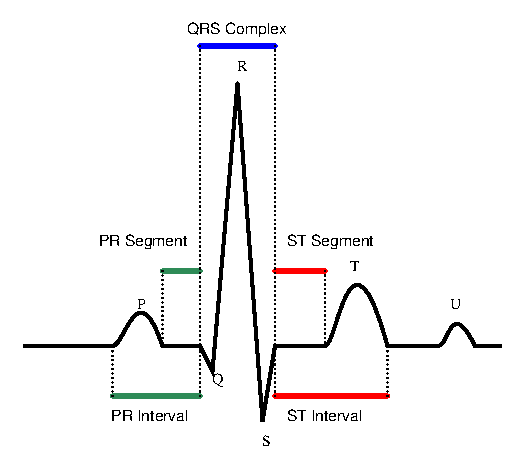
\includegraphics[scale=0.80]{./Figures/ElectroCardioGraphy.ps}
		\caption{Electrocardiograph (ECG) Signal.}
		\label{fig:ECG}
	\end{center}
\end{figure}


\section{Level cross sampling scheme}

\par
\hspace{1.2cm} The principle of level crossing ADC's is the dual case of Nyquist ADC's. In Nyquist ADC's the time instants are perfectly known and samples of amplitude are quantized, where as in case of level crossing ADC's the amplitude levels are known and the samples of time are quantized. Fig.~\ref{fig:LCS} shows the level cross sampling scheme~\cite{1595684}. In level crossing ADC's the occurrence of samples depend on signal amplitude variations, this sampling scheme removes the conversion of redundant samples or samples without any relevant information when the analog signal is quiet. Therefore, it leads to a compression of digital samples and a reduction in the activity of the circuit.

\begin{figure}[ht]
	\begin{center}
		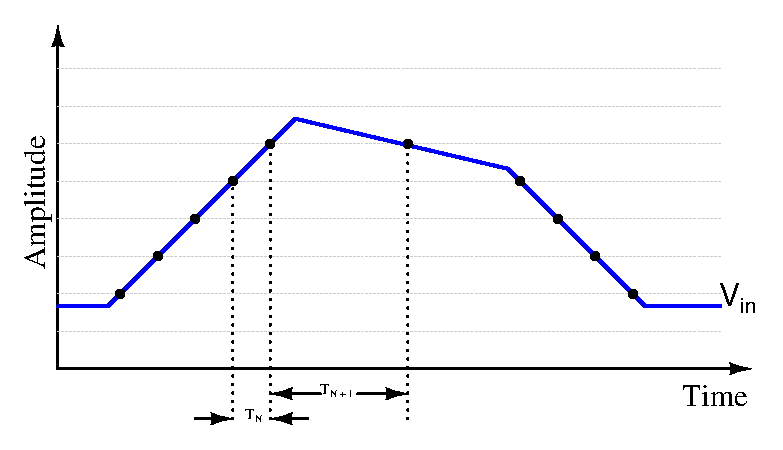
\includegraphics[scale=0.75]{./Figures/LevelCrossing.ps}
		\caption{Principle of the level crossing sampling scheme. }
		\label{fig:LCS}
	\end{center}
\end{figure}

\par
\hspace{0.6cm} In level crossing ADC's for M-bits resolution it requires $2^M-1$ quantization levels are regularly disposed along the amplitude range of the input signal $V_{in}$. A sample is taken only when the analog input signal $V_{in}$ crosses one of quantization levels. Contrary to classical Nyquist sampling, samples are not regularly spaced out in time, because it depends on the variation of input signal $V_{in}$~\cite{allier2005asynchronous}. Table.~\ref{tab:DNL} shows difference between Nyquist sampling and level cross sampling schemes. Level cross sampling is best suited for asynchronous and low power applications~\cite{allier2003new}.

\begin{table}[t]
	\caption{Difference Between Nyquist \& Level Cross Sampling Schemes}
	\label{tab:DNL}
	\begin{center}
	\resizebox{10cm}{!}{
		\begin{tabular}{c|c|c|}
			\cline {2-3} %\hline
		 	&{Nyquist Sampling} & {Level Cross Sampling} \\ \hline
			\multicolumn {1}{|c|} {Conversion Trigger} &   {Clock} &  {Level Crossing} \\ \hline
			\multicolumn {1}{|c|} {Amplitude} &  {Quantized} &  {Exact Value} \\ \hline
			\multicolumn {1}{|c|} {Time} &  {Exact Value} &  {Quantized} \\ \hline
			\multicolumn {1}{|c|} {SNR Dependency} &  {Number of Bits} &  {Timer Period} \\ \hline
			\multicolumn {1}{|c|} {Converter Output} &  {Amplitude} &  {Amplitude \& Time} \\ \hline
		\end{tabular} }	
	\end{center}
\end{table}

\par
\hspace{0.6cm} Level-cross sampling scheme is the dual of the Nyquist sampling scheme. In Nyquist \mbox{ADC's} the samples are taken at fixed intervals of time with reference to the clock signal. The minimum clock signal is chosen to be twice the maximum frequency of the analog input signal. For signals in which the frequency content is very low for most of the time, with rare occurrences of high frequency contents, it leads to over sampling. Hence, taking samples at regular intervals of time unnecessarily increases circuit activity, which in turn increases the power consumption~\cite{sayiner1996level}.

\par
\hspace{0.6cm} 	\mbox{LC-ADC's} are driven by the level-crossing rather than by clock ie., the conversion process triggers when the analog input crosses any of the quantization levels, these are best suited for asynchronous and low power applications~\cite{allier2003new}. The level-cross sampling scheme can be understood by using Fig.~\ref{fig:ECG}, which shows a typical ECG signal. The dotted lines represent quantization levels. 


\par
\hspace{0.6cm} The level-cross sampling scheme can be understood by using Fig.~\ref{fig:ECG}, which shows a typical ECG signal. The dotted lines represent quantization levels. In \mbox{LC-ADC's}, for an N-bit hardware resolution, $2^{N}-1$ quantization levels are regularly spaced along the amplitude range of the analog input signal. A sample is taken only when the analog input signal crosses any one of the $2^{N}-1$ quantization levels. The shape of the analog input signal can be preserved by calculating the time difference between two successive samples. Thus, outputs from \mbox{LC-ADC's} are amplitude and time data pairs, unlike that of Nyquist \mbox{ADC's} where the output consists of only amplitude data. Table.~\ref{tab:DNL} shows the difference between Nyquist and Level-Crossing sampling schemes.


\begin{figure}[ht]
	\begin{center}
		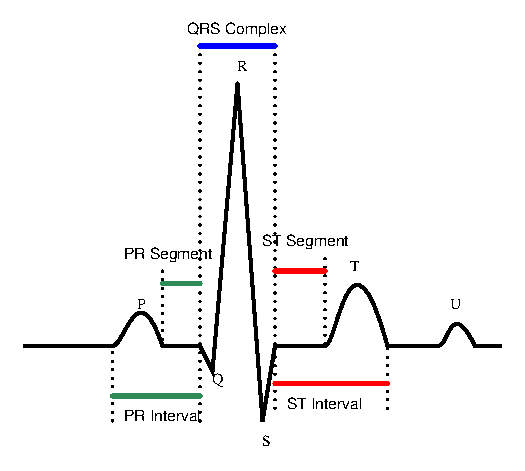
\includegraphics[height=8.5 cm, angle=270]{./Figures/ECG.ps}
		\caption{level-cross sampling scheme for an ECG signal}
		\label{fig:ECGS}
	\end{center}
\end{figure}


\par
\hspace{0.6cm} In \mbox{LC-ADC's}, for an N-bit hardware resolution, $2^{N}-1$ quantization levels are regularly spaced along the amplitude range of the analog input signal. A sample is taken only when the analog input signal crosses any one of the $2^{N}-1$ quantization levels. The shape of the analog input signal can be preserved by calculating the time difference between two successive samples. Thus, outputs from \mbox{LC-ADC's} are amplitude and time data pairs, unlike that of Nyquist \mbox{ADC's} where the output consists of only amplitude data. Table.~\ref{tab:DNL} shows the difference between Nyquist and Level-Crossing sampling schemes. 

\par
\hspace{0.6cm} The time taken from analog input crossing one of the quantization levels to complete conversion is called loop delay. The loop delay of the LC-ADC decides the maximum input signal frequency which can be tracked without slope overload error by the ADC. The proposed architecture is aimed to reduce this loop delay so that it can track high frequency components in input analog signal without slope overloading error.

\par
\hspace{1.2cm} There are some drawbacks in level cross sampling ADC's, timer will define the resolution of the level crossing ADC's, which requires separate high speed clock generation circuit for timer to calculate the difference between present sample and previous sample. When tracking analog input signal it follows linear successive approximation which can't track sharp raise and fall edges in analog input signal~\cite{5672382}. When designing level cross A to D converters one must know the statistical properties of the signal clearly~\cite{allier2005asynchronous}, once designed for particular application can't be used for other application effectively. In this proposed work an attempt has been made to overcome these drawback of the level cross sampling A to D converters.


\section{Organization of the Report}

\par
\hspace{1.2cm} The remainder of the report is organized as follows. Chapter 2 gives a brief overview on literature review of the level crossing ADC architectures. Chapter 3 describes the  proposed ADC architectures, its principle is based on a level cross sampling scheme that allow reduction in activity of the circuit. Chapter 4 describes conclusion and future work.




